\documentclass[handout, c, 11pt, xcolor=svgnames, hyperref={colorlinks,citecolor=DeepPink4,linkcolor=DarkRed,urlcolor=DarkBlue}]{beamer} % t aligns all blocks and text to the top (default is aligned to center)
%\usepackage{pgfpages}
%\pgfpagesuselayout{4 on 1}[a4paper, border shrink=5mm, landscape]


\usepackage[english, german]{babel}
\usepackage[latin1]{inputenc}
\usepackage[T1]{fontenc}

\mode<presentation> {
	
	% The Beamer class comes with a number of default slide themes
	% which change the colors and layouts of slides. Below this is a list
	% of all the themes, uncomment each in turn to see what they look like.
	
	%\usetheme{default}
	%\usetheme{AnnArbor}
	%\usetheme{Antibes}
	%\usetheme{Bergen}
	%\usetheme{Berkeley}
	%\usetheme{Berlin}
	%\usetheme{Boadilla}
	\usetheme{CambridgeUS}
	%\usetheme{Copenhagen}
	%\usetheme{Darmstadt}
	%\usetheme{Dresden}
	%\usetheme{Frankfurt}
	%\usetheme{Goettingen}
	%\usetheme{Hannover}
	%\usetheme{Ilmenau}
	%\usetheme{JuanLesPins}
	%\usetheme{Luebeck}
	%\usetheme{Madrid}
	%\usetheme{Malmoe}
	%\usetheme{Marburg}
	%\usetheme{Montpellier}
	%\usetheme{PaloAlto}
	%\usetheme{Pittsburgh}
	%\usetheme{Rochester}
	%\usetheme{Singapore}
	%\usetheme{Szeged}
	%\usetheme{Warsaw}
	
	% As well as themes, the Beamer class has a number of color themes
	% for any slide theme. Uncomment each of these in turn to see how it
	% changes the colors of your current slide theme.
	
	%\usecolortheme{albatross}
	%\usecolortheme{beaver}
	%\usecolortheme{beetle}
	%\usecolortheme{crane}
	%\usecolortheme{dolphin}
	%\usecolortheme{dove}
	%\usecolortheme{fly}
	%\usecolortheme{lily}
	%\usecolortheme{orchid}
	%\usecolortheme{rose}
	%\usecolortheme{seagull}
	%\usecolortheme{seahorse}
	%\usecolortheme{whale}
	%\usecolortheme{wolverine}
	
	\usefonttheme{professionalfonts}
	
	\usepackage{times}
	\usepackage{tikz}
	\usetikzlibrary{arrows,shapes}
	
	%\setbeamertemplate{footline} % To remove the footer line in all slides uncomment this line
	%\setbeamertemplate{footline}[page number] % To replace the footer line in all slides with a simple slide count uncomment this line
	\setbeamertemplate{headline} % to remove header with navigation tree
	
	\setbeamertemplate{navigation symbols}{} % To remove the navigation symbols from the bottom of all slides uncomment this line
}

\usepackage{amsmath,mathtools}
\usetikzlibrary{matrix, fit, backgrounds}

\usepackage{graphicx} % Allows including images
\usepackage{booktabs} % Allows the use of \toprule, \midrule and \bottomrule in tables
\usepackage{subcaption}
\usepackage{tabularx}

\usetikzlibrary{mindmap,trees,shadows,backgrounds}

%\tikzset{every node/.append style={scale=0.6}}    

\usepackage{array,multirow}
\usepackage{changepage}

\usepackage[backend=biber, style=authoryear-comp, citestyle=authoryear-comp, firstinits=true, url=false, doi=false, eprint=false, dashed=false, maxbibnames=99]{biblatex}
\addbibresource{bib.bib}

%----------------------------------------------------------------------------------------
%	TITLE PAGE
%----------------------------------------------------------------------------------------

\title[Webinar for ISDS R Group]{Building meaningful machine learning models for disease prediction} % The short title appears at the bottom of every slide, the full title is only on the title page

\author{Dr Shirin Glander} % Your name
\institute[] % Your institution as it will appear on the bottom of every slide, may be shorthand to save space
{
	Dep. of Genetic Epidemiology \\
	Institute of Human Genetics \\
	University of M\"unster
	
	\vspace{0.5cm} 
	
	\href{mailto:shirin.glander@wwu.de}{shirin.glander@wwu.de} \\
	
	\vspace{0.5cm} 
	
	\href{https://shiring.github.io}{https://shiring.github.io} \\
	
	\href{https://github.com/ShirinG}{https://github.com/ShirinG}
	
}
\date{31.03.2017
	\vspace{0.5cm}
} % Date, can be changed to a custom date

\AtBeginSection[]{
	\begin{frame}
		\vfill
		\centering
		\begin{beamercolorbox}[sep=8pt,center,shadow=true,rounded=true]{title}
			\usebeamerfont{title}\insertsectionhead\par%
		\end{beamercolorbox}
		\vfill
	\end{frame}
}

\renewcommand{\thefootnote}{$\star$} 

\begin{document}
	
	\begin{frame}
		\titlepage % Print the title page as the first slide
		
		%Dr Shirin Glander will go over her work on building machine-learning models to predict the course of different diseases. She will go over building a model, evaluating its performance, and answering or addressing different disease related questions using machine learning. Her talk will cover the theory of machine learning as it is applied using R. 
	\end{frame}
	
	\begin{frame}[c]
		\frametitle{Table of contents}
		
			\tableofcontents[hideallsubsections]

	\end{frame}

\begin{frame}
	\frametitle{About me}
	
	\begin{columns}
		\column{0.15\textwidth}	
	
		\column{0.8\textwidth}	
	\begin{itemize}
		\item[2005 - 2011] BSc and MSc of Science in Biology \\
							Evolutionary genetics, \\ immune memory in Drosophila \\[5mm]
		\item[2011 - 2015] PhD in Biology \\
							Is the immune system of plants required to adapt to flowering time change? \\[5mm]
		\item[since 2015] Bioinformatics Postdoc \\
							Autoinflammatory diseases \& innate immunity \\
							Next Generation Sequencing
	\end{itemize}

	\column{0.05\textwidth}	
	
	\begin{tikzpicture}[remember picture,overlay]
	\node[xshift=-2cm,yshift=-2.5cm] at (current page.north east) {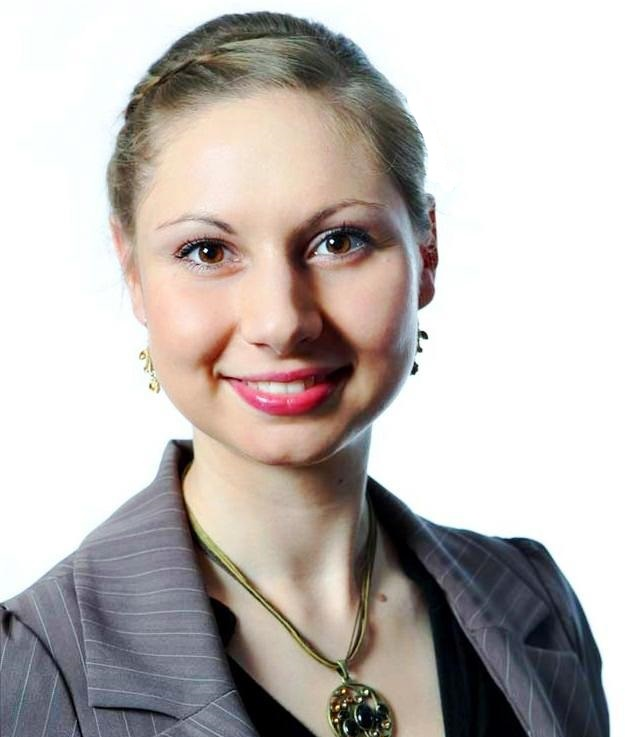
\includegraphics[width=3cm]{images/Bewerbungsfoto}};
	\end{tikzpicture}

	\end{columns}
\end{frame}

%%%%%%%%%%%%%%%%%%%%%

\section{What makes a model meaningful?}

\begin{frame}
	\frametitle{\textsl{Meaningful} models}
	
	\begin{itemize}
		\item answer the question(s) posed...
		\item ... with sufficient accuracy to be trustworthy
	\end{itemize}

\vspace{0.6cm}

	\begin{center}
		{\Large \alert{Accuracy depends on the problem!}}
		
		\vspace{1cm}
		
		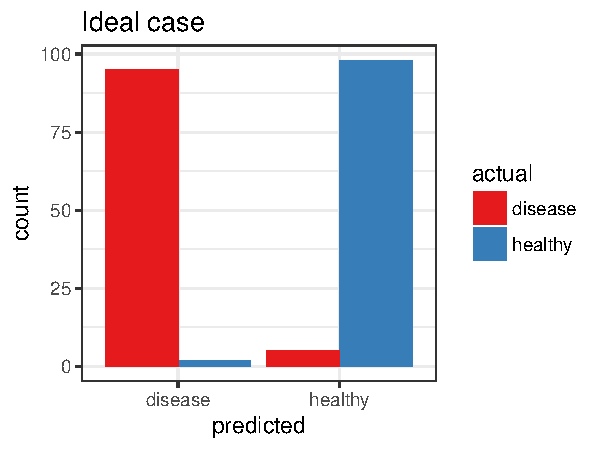
\includegraphics[width=0.33\textwidth]{images/meaningful_1}
		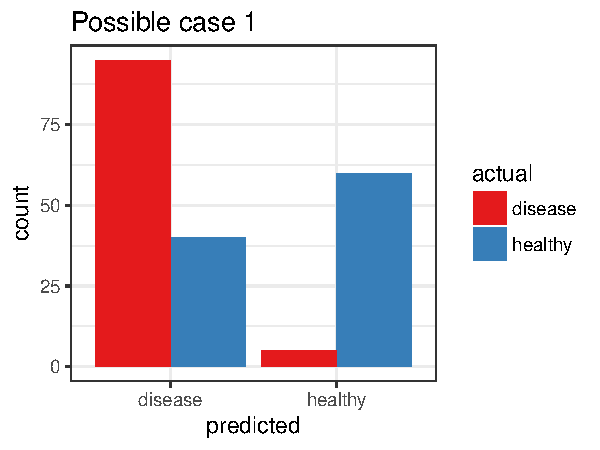
\includegraphics[width=0.33\textwidth]{images/meaningful_2}
		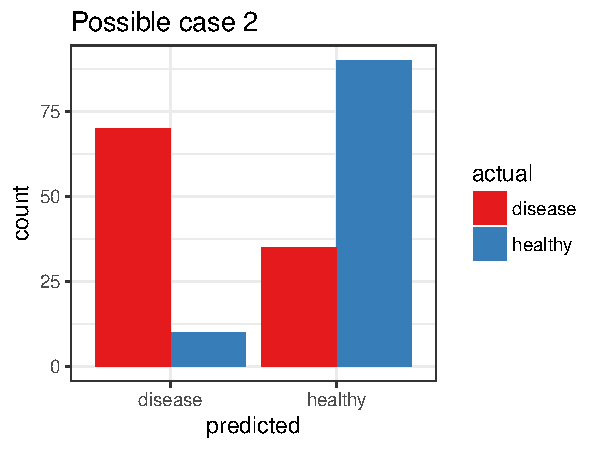
\includegraphics[width=0.33\textwidth]{images/meaningful_3}
	\end{center}
	
	
\end{frame}


%%%%%%%%%%%%%%%%%%%%%

\section{Machine Learning (ML) in disease modeling}

%publications

\begin{frame}
	
	\footfullcite{doi:10.1146/annurev.bioeng.8.061505.095802}
	%\footcite{doi:10.1146/annurev.bioeng.8.061505.095802}
	
\end{frame}

%%%%%%%%%%%%%%%%%%%%%

\section{A quick recap of ML basics}

\subsection{Supervised vs Unsupervised algorithms}

\subsection{Classification vs Regression}

\subsection{Features}

% feature engineering
% feature selection
% factorial vs numeric
% preprocessing

\subsection{Training, validation and test data}

\subsection{Cross-validation}

\subsection{Missing data}

\subsection{Grid Search}

%imputation


%%%%%%%%%%%%%%%%%%%%%

\section{How to build ML models in R}

\begin{frame}
	\frametitle{Session setup}
	
	Code will be available on \href{https://shiring.github.io}{my website} and on \href{https://github.com/ShirinG/Webinar_ML_for_disease}{Github}
	
	Breast cancer Wisconsin dataset
	
	caret package
	
	h2o package
\end{frame}

\subsection{Get to know your data}

\begin{frame}
	\frametitle{Distribution}
	
	\begin{center}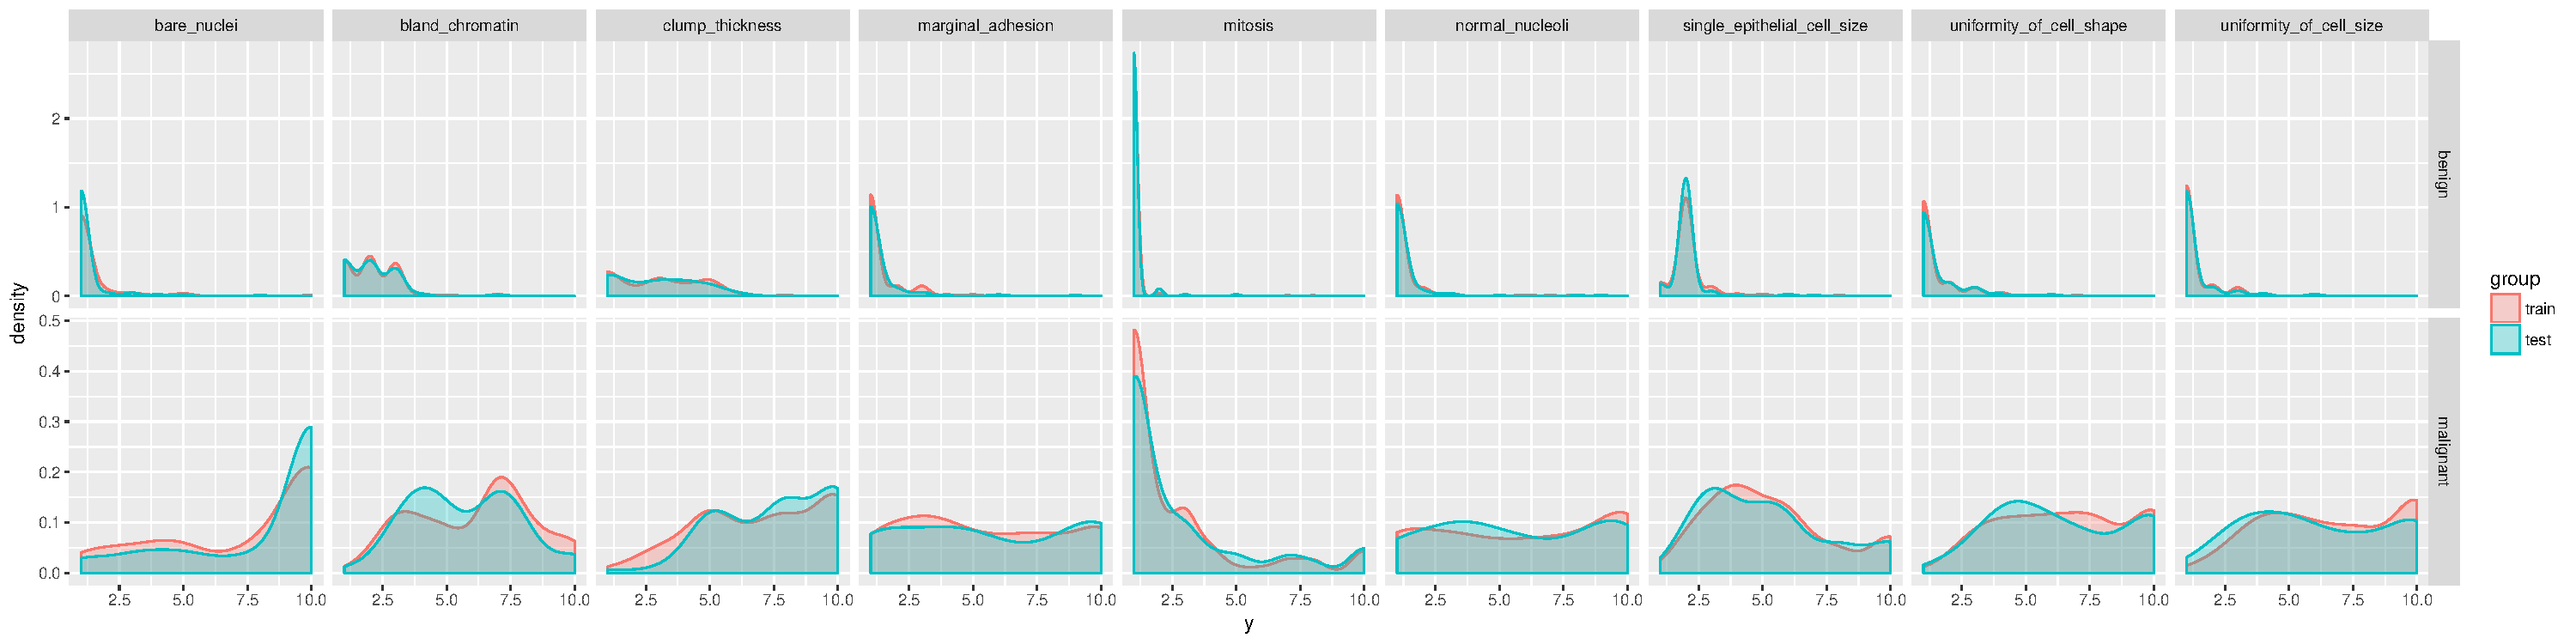
\includegraphics[width=1\textwidth]{webinar_code_files/figure-latex/unnamed-chunk-6-1} \end{center}
\end{frame}


\subsection{Classification}

\subsubsection{Tree based models}

\begin{frame}
	\frametitle{Decision trees}
	
	\begin{center}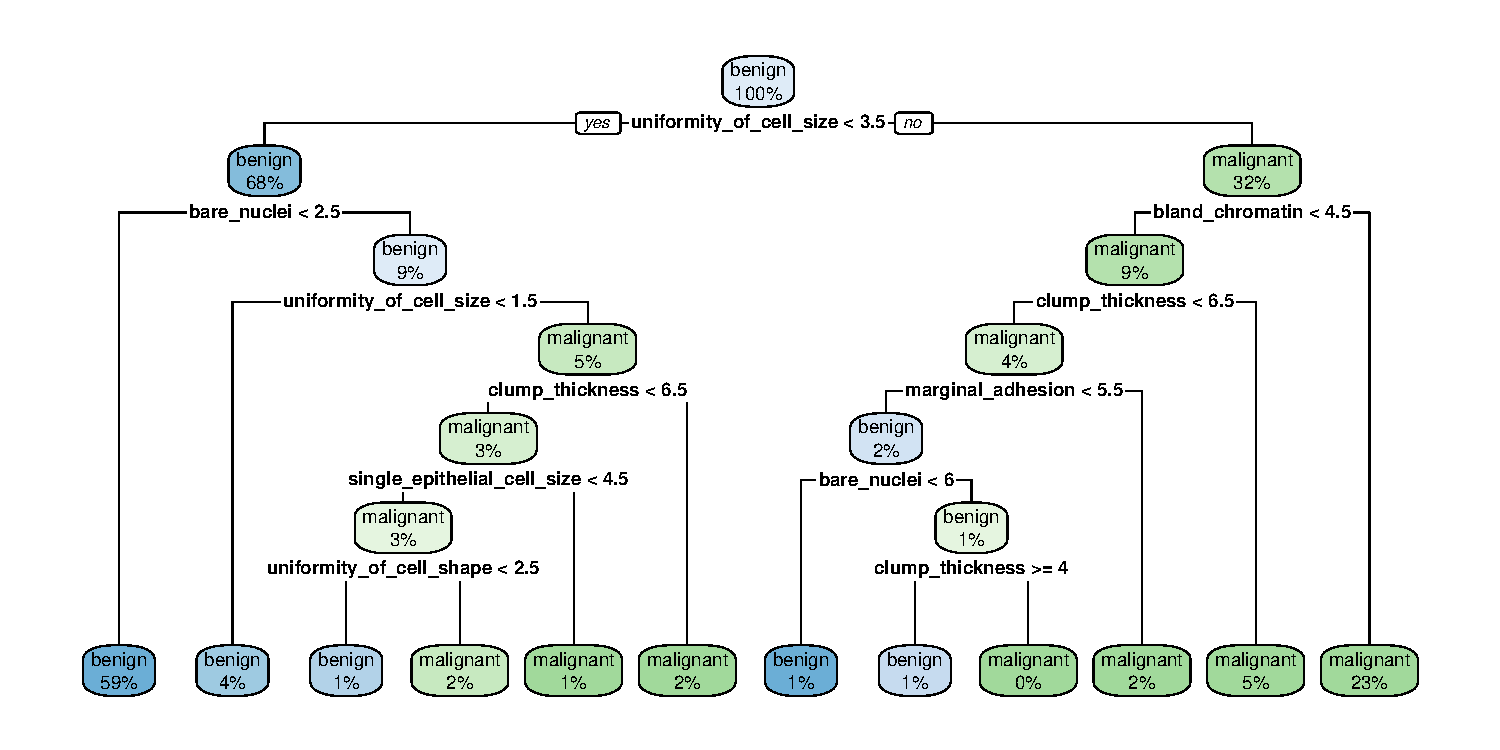
\includegraphics[width=1\textwidth]{webinar_code_files/figure-latex/unnamed-chunk-12-1} \end{center}
	
\end{frame}

\begin{frame}
	\frametitle{Random Forest}
	
	
\end{frame}

\begin{frame}
	\frametitle{Feature importance}
	
	\begin{center}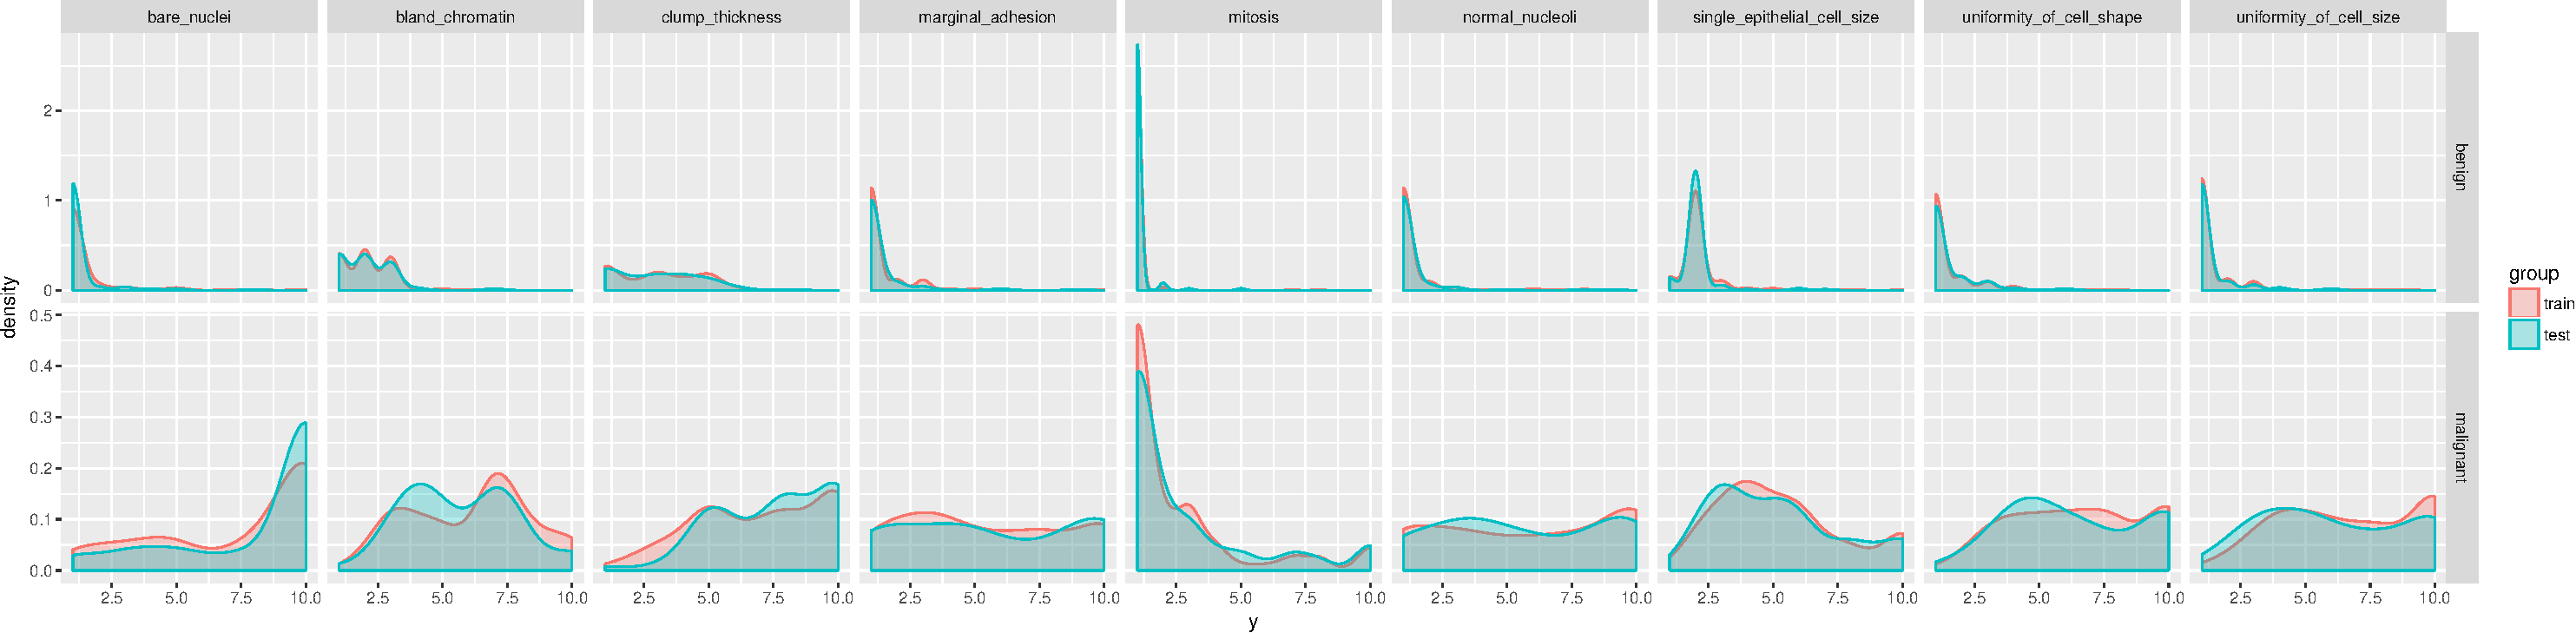
\includegraphics[width=1\textwidth]{webinar_code_files/figure-latex/unnamed-chunk-11-1.pdf} \end{center}
\end{frame}

\subsection{Regression}

\subsubsection{Linear Models}

\begin{frame}
	\frametitle{(Generalized) Linear Models}
	
	\begin{center}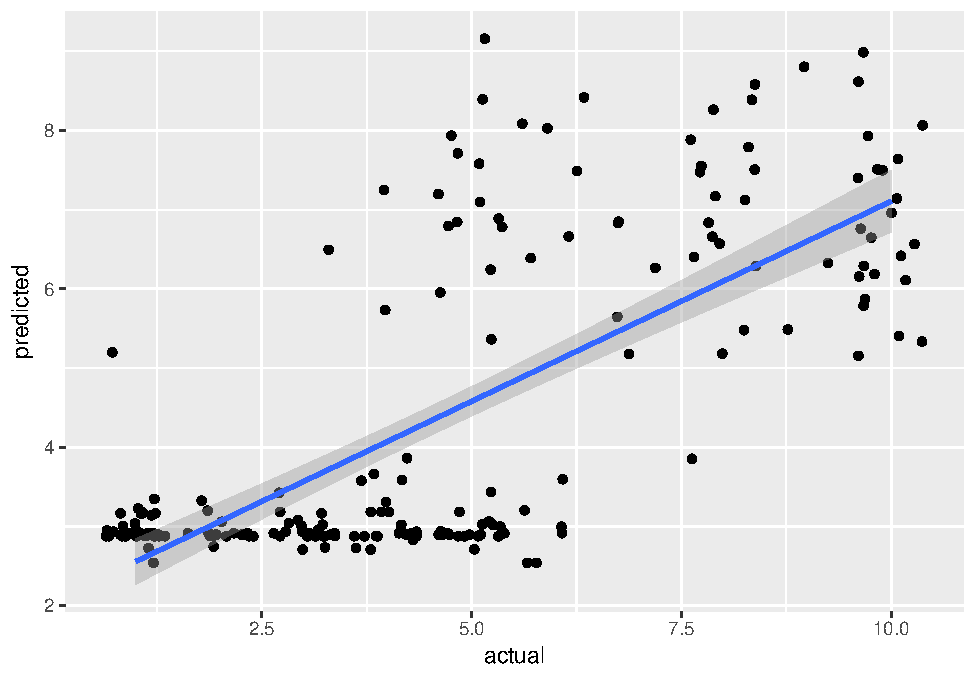
\includegraphics[width=1\textwidth]{webinar_code_files/figure-latex/unnamed-chunk-21-1.pdf} \end{center}
\end{frame}

\subsubsection{Deep learning with neural network}

% h2o


%%%%%%%%%%%%%%%%%%%%%

\section{Evaluating ML model performance}

\subsection{Validation vs test set performance}

\begin{frame}
	\frametitle{AUC and MSE}
	
	\begin{center}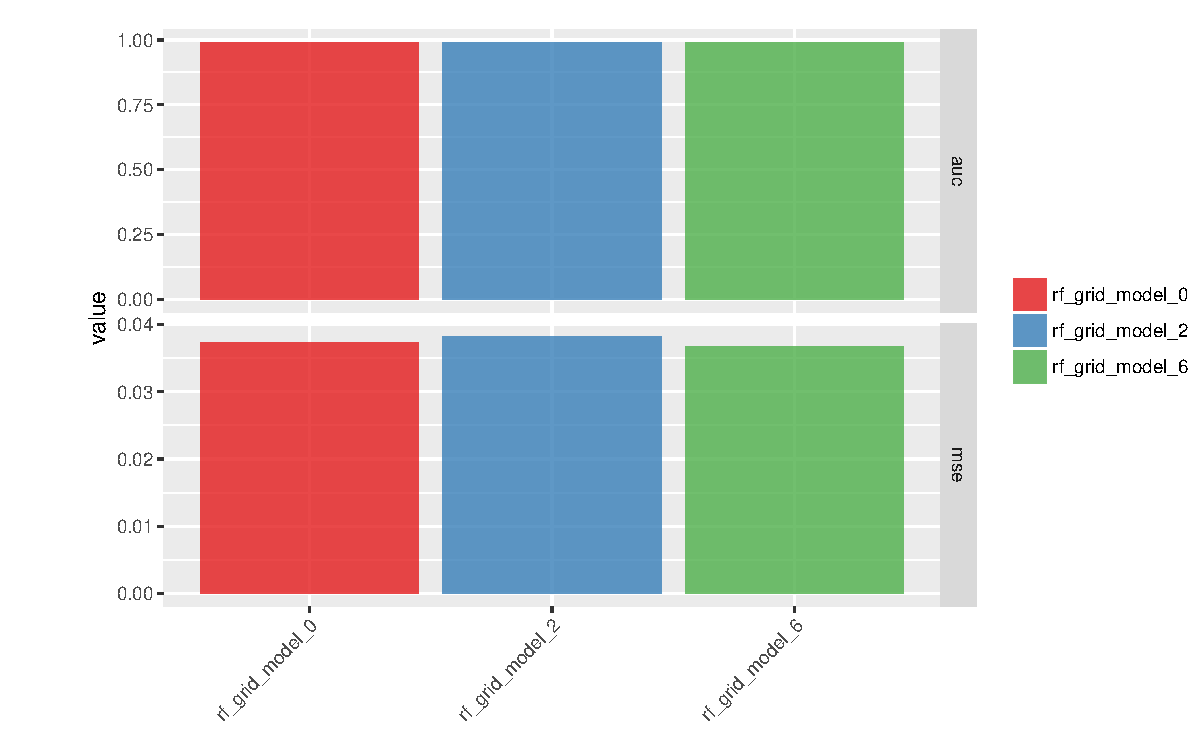
\includegraphics[width=1\textwidth]{webinar_code_files/figure-latex/unnamed-chunk-29-1.pdf} \end{center}
	
	\begin{center}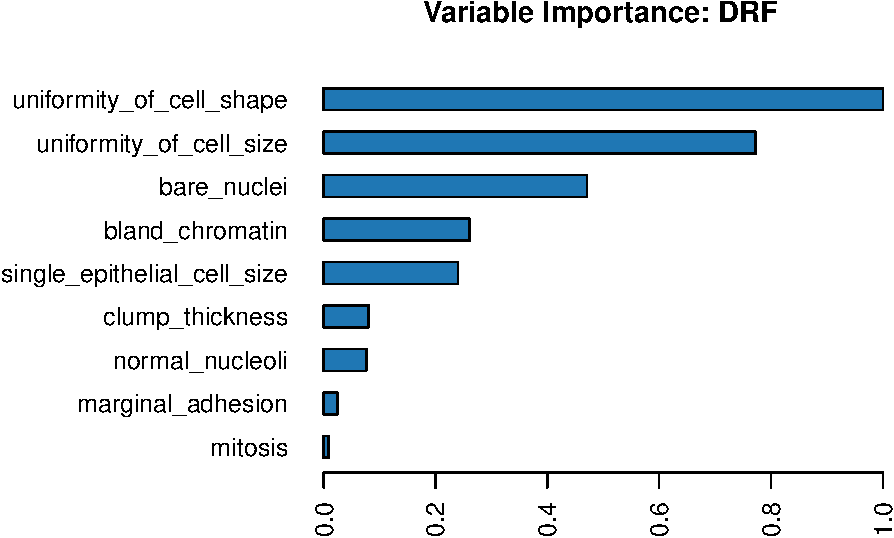
\includegraphics[width=1\textwidth]{webinar_code_files/figure-latex/unnamed-chunk-42-1} \end{center}
\end{frame}

\begin{frame}
	\frametitle{Predictions on test data}
	
	\begin{center}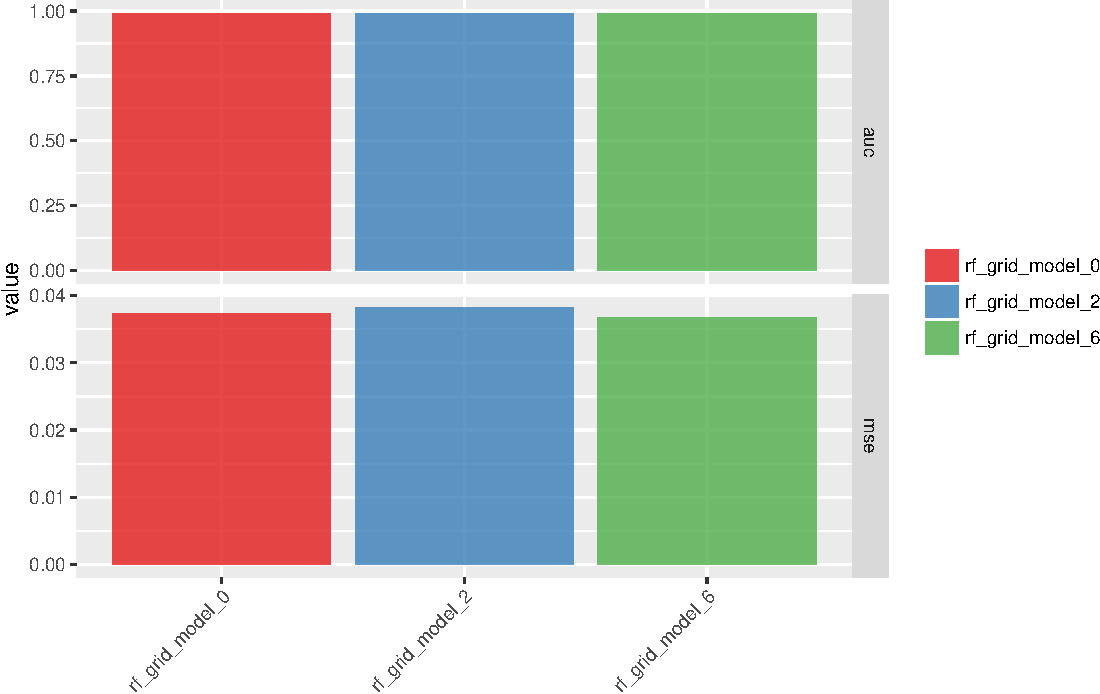
\includegraphics[width=1\textwidth]{webinar_code_files/figure-latex/unnamed-chunk-31-1.pdf}
	
	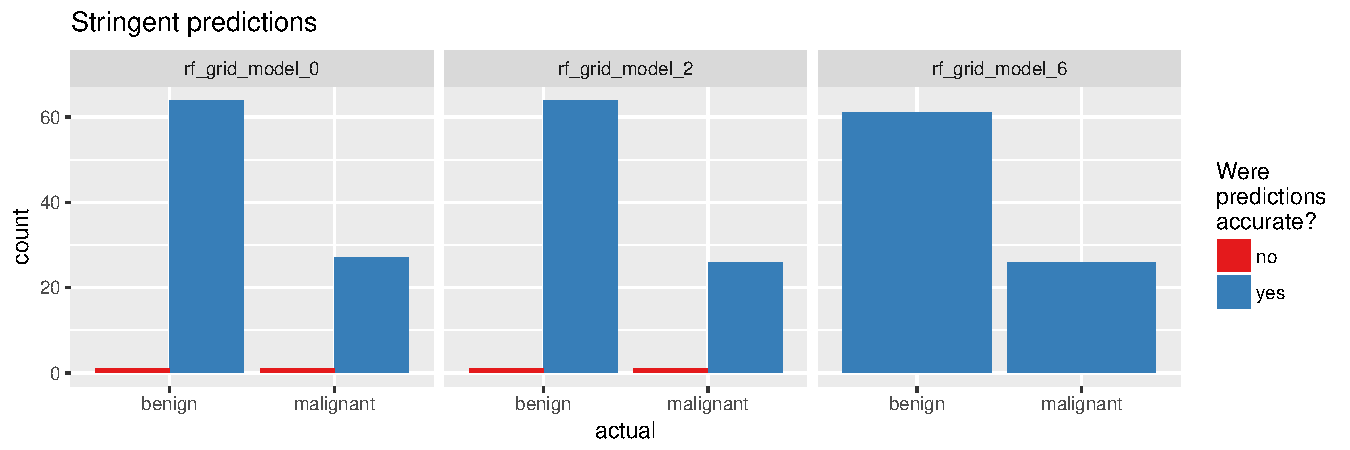
\includegraphics[width=1\textwidth]{webinar_code_files/figure-latex/unnamed-chunk-31-2.pdf} \end{center}
\end{frame}

% accuracy
% Kappa


%%%%%%%%%%%%%%%%%%%%%

\begin{frame}[plain, c]
	
	\begin{center}
	\usebeamerfont*{frametitle} \usebeamercolor[fg]{frametitle} {\Huge \textbf{Thank you for your attention!}}
	\end{center}

	\vspace{0.5cm}

	\begin{center}
		\usebeamerfont*{frametitle} {\huge Questions?}
	\end{center}

	\vspace{0.5cm}
	
	Slides and code will be available on Github: \href{https://github.com/ShirinG/Webinar_ML_for_disease}{https://github.com/ShirinG/Webinar\_ML\_for\_disease} \\
	
	\vspace{0.5cm}
	
	Code will also be on my website: \href{https://shiring.github.io}{https://shiring.github.io} \\
	
	\vspace{0.5cm}
	
	\href{mailto:shirin.glander@wwu.de}{shirin.glander@wwu.de} \\
	
\end{frame}

\end{document}